%!TEX program = xelatex
% LaTeX 数学符号与语法快速参考教程
% 基于 LaTeX 备忘清单转换

\documentclass[cn,hazy,blue,14pt,screen]{elegantnote}

\title{LaTeX 数学符号与语法快速参考}
\author{基于 LaTeX Cheatsheet}
\date{\zhdate{2026/02/02}}

% 💡 额外加载的宏包
\usepackage{booktabs}  % 更美观的表格
\usepackage{multirow}  % 跨行单元格
\usepackage{cancel}    % 删除线效果
\usepackage[normalem]{ulem}  % 文字删除线
\usepackage{amssymb}   % 额外数学符号 (digamma, varkappa)

\begin{document}

\maketitle

\tableofcontents
\clearpage

%% =============================================================================
%% 文档引言
%% =============================================================================
\section*{前言}
\addcontentsline{toc}{section}{前言}

\begin{center}
\begin{tikzpicture}
  \node[fill=ecolor!10, draw=ecolor, rounded corners=8pt, 
        inner sep=15pt, text width=0.9\linewidth] {
    \faBookOpen\hspace{0.5em}\textbf{关于本教程}
    
    \smallskip
    本教程汇集了 \LaTeX{} 数学排版中最常用的符号、语法和技巧。
    无论你是刚接触 \LaTeX{} 的新手,还是需要快速查阅的老用户,
    这份参考都能帮助你高效地完成数学公式排版。
    
    \smallskip
    {\small\color{gray} 每个示例都提供「代码」与「效果」的直观对比,让学习更加轻松。}
  };
\end{tikzpicture}
\end{center}

%% =============================================================================
%% 第一部分:入门
%% =============================================================================
\section{入门}

\LaTeX{} 是一种基于 \TeX{} 的排版系统,广泛用于学术论文、技术文档和书籍的排版。
本章将介绍数学公式排版的基础知识,帮助你快速上手。

\subsection{数学模式}

\LaTeX{} 中的数学公式有两种基本形式:

\begin{itemize}
  \item \textbf{行内公式}:使用 \verb|$...$| 或 \verb|\(...\)| 包裹,公式与文字融为一体
  \item \textbf{行间公式}:使用 \verb|$$...$$| 或 \verb|\[...\]| 包裹,公式独占一行居中显示
\end{itemize}

\begin{example}[行内公式]
代码:\verb|质能方程 $E=mc^2$ 是物理学的基础公式。|

效果:质能方程 $E=mc^2$ 是物理学的基础公式。
\end{example}

\begin{example}[行间公式]
代码:
\begin{lstlisting}
\[ f(x) = \int_{-\infty}^{\infty} \hat{f}(\xi) e^{2\pi i\xi x} d\xi \]
\end{lstlisting}

效果:
\[ f(x) = \int_{-\infty}^{\infty} \hat{f}(\xi) e^{2\pi i\xi x} d\xi \]
\end{example}

\begin{note}
行间公式更适合展示重要公式,而行内公式适合嵌入文字中的简短表达式。
推荐使用 \verb|\[...\]| 而非 \verb|$$...$$|,前者是 \LaTeX{} 标准写法。
\end{note}

%% =============================================================================
%% 核心对比:行内 vs 行间
%% =============================================================================
\subsection{公式显示效果对比}

\infobox[tip]{同一个公式在行内和行间模式下显示效果有显著差异,尤其是分数和积分。}

\begin{table}[htbp]
\centering
\caption{行内模式 vs 行间模式显示对比}
\begin{tabular}{lcc}
\toprule
公式类型 & 行内模式 & 行间模式 \\
\midrule
分数 & $\frac{a}{b}$ & $\displaystyle\frac{a}{b}$ \\[8pt]
求和 & $\sum_{i=1}^{n} i$ & $\displaystyle\sum_{i=1}^{n} i$ \\[8pt]
积分 & $\int_0^1 x\,dx$ & $\displaystyle\int_0^1 x\,dx$ \\[8pt]
极限 & $\lim_{x\to 0} f(x)$ & $\displaystyle\lim_{x\to 0} f(x)$ \\
\bottomrule
\end{tabular}
\end{table}

\begin{example}[强制切换显示样式]
使用 \verb|\displaystyle| 在行内强制大尺寸显示:

行内大分数:$\displaystyle\frac{a}{b}$

代码:\verb|$\displaystyle\frac{a}{b}$|
\end{example}

%% =============================================================================
%% 第二部分:希腊字母
%% =============================================================================
\clearpage
\section{希腊字母}

希腊字母在数学和物理中无处不在——从 $\alpha, \beta, \gamma$ 表示角度,
到 $\Omega$ 表示电阻,再到 $\pi$ 这个神奇的圆周率。掌握这些字母的输入方式是使用 \LaTeX{} 的第一步。

\subsection{小写希腊字母}

\begin{table}[htbp]
\centering
\caption{小写希腊字母速查表}
\begin{tabular}{llllllll}
\toprule
预览 & 代码 & 预览 & 代码 & 预览 & 代码 & 预览 & 代码 \\
\midrule
$\alpha$ & \verb|\alpha| & $\beta$ & \verb|\beta| & $\gamma$ & \verb|\gamma| & $\delta$ & \verb|\delta| \\
$\epsilon$ & \verb|\epsilon| & $\zeta$ & \verb|\zeta| & $\eta$ & \verb|\eta| & $\theta$ & \verb|\theta| \\
$\iota$ & \verb|\iota| & $\kappa$ & \verb|\kappa| & $\lambda$ & \verb|\lambda| & $\mu$ & \verb|\mu| \\
$\nu$ & \verb|\nu| & $\xi$ & \verb|\xi| & $\pi$ & \verb|\pi| & $\rho$ & \verb|\rho| \\
$\sigma$ & \verb|\sigma| & $\tau$ & \verb|\tau| & $\upsilon$ & \verb|\upsilon| & $\phi$ & \verb|\phi| \\
$\chi$ & \verb|\chi| & $\psi$ & \verb|\psi| & $\omega$ & \verb|\omega| & & \\
\bottomrule
\end{tabular}
\end{table}

\subsection{变体形式}

部分希腊字母有变体形式,在不同场景下使用:

\begin{table}[htbp]
\centering
\caption{希腊字母变体对比}
\begin{tabular}{llllp{4cm}}
\toprule
标准形式 & 代码 & 变体形式 & 代码 & 应用场景 \\
\midrule
$\epsilon$ & \verb|\epsilon| & $\varepsilon$ & \verb|\varepsilon| & 分析学常用 $\varepsilon$ \\
$\theta$ & \verb|\theta| & $\vartheta$ & \verb|\vartheta| & 手写体风格 \\
$\phi$ & \verb|\phi| & $\varphi$ & \verb|\varphi| & $\varphi$ 表示黄金比例 \\
$\rho$ & \verb|\rho| & $\varrho$ & \verb|\varrho| & 带卷曲尾巴 \\
$\sigma$ & \verb|\sigma| & $\varsigma$ & \verb|\varsigma| & 希腊词尾形式 \\
\bottomrule
\end{tabular}
\end{table}

\subsection{大写希腊字母}

\begin{table}[htbp]
\centering
\caption{大写希腊字母(仅显示与拉丁字母不同的)}
\begin{tabular}{llllllll}
\toprule
预览 & 代码 & 预览 & 代码 & 预览 & 代码 & 预览 & 代码 \\
\midrule
$\Gamma$ & \verb|\Gamma| & $\Delta$ & \verb|\Delta| & $\Theta$ & \verb|\Theta| & $\Lambda$ & \verb|\Lambda| \\
$\Xi$ & \verb|\Xi| & $\Pi$ & \verb|\Pi| & $\Sigma$ & \verb|\Sigma| & $\Upsilon$ & \verb|\Upsilon| \\
$\Phi$ & \verb|\Phi| & $\Psi$ & \verb|\Psi| & $\Omega$ & \verb|\Omega| & & \\
\bottomrule
\end{tabular}
\end{table}

\begin{note}
大写希腊字母中 A, B, E, H, I, K, M, N, O, P, T, X, Z 与拉丁字母相同,
因此直接输入即可,无需特殊命令。
\end{note}

%% =============================================================================
%% 第三部分:上下标与修饰符号
%% =============================================================================
\clearpage
\section{上下标与修饰符号}

掌握了希腊字母后,下一步是学习如何给符号添加上下标和各种修饰——
从简单的幂指数到复杂的向量表示,这些语法是构建公式的基础砖块。

\subsection{上标与下标}

\begin{table}[htbp]
\centering
\caption{上下标语法}
\begin{tabular}{llll}
\toprule
效果 & 代码 & 效果 & 代码 \\
\midrule
$a^2$ & \verb|a^2| & $a_i$ & \verb|a_i| \\
$a^{n+1}$ & \verb|a^{n+1}| & $a_{i,j}$ & \verb|a_{i,j}| \\
$x_n^2$ & \verb|x_n^2| & ${}_1^2X_3^4$ & \verb|{}_1^2X_3^4| \\
\bottomrule
\end{tabular}
\end{table}

\infobox[warning]{多字符上下标必须用花括号包裹!\texttt{a\^{}10} 显示为 $a^10$(只有1是上标),而 \texttt{a\^{}\{10\}} 才正确显示为 $a^{10}$。}

\subsection{重音与修饰符号}

数学中常用重音符号表示特殊含义,如导数、平均值、向量等:

\begin{table}[htbp]
\centering
\caption{常用重音符号}
\begin{tabular}{llllll}
\toprule
效果 & 代码 & 用途 & 效果 & 代码 & 用途 \\
\midrule
$\hat{a}$ & \verb|\hat{a}| & 估计量 & $\widehat{AB}$ & \verb|\widehat{AB}| & 宽帽子 \\
$\bar{x}$ & \verb|\bar{x}| & 平均值 & $\overline{xyz}$ & \verb|\overline{xyz}| & 共轭 \\
$\vec{v}$ & \verb|\vec{v}| & 向量 & $\overrightarrow{AB}$ & \verb|\overrightarrow{AB}| & 有向线段 \\
$\dot{x}$ & \verb|\dot{x}| & 一阶导 & $\ddot{x}$ & \verb|\ddot{x}| & 二阶导 \\
$\tilde{a}$ & \verb|\tilde{a}| & 近似 & $\widetilde{abc}$ & \verb|\widetilde{abc}| & 宽波浪 \\
\bottomrule
\end{tabular}
\end{table}

\begin{example}[物理中的典型应用]
\begin{align*}
\text{牛顿第二定律:} \quad & \vec{F} = m\ddot{\vec{r}} \\
\text{样本均值:} \quad & \bar{X} = \frac{1}{n}\sum_{i=1}^{n} X_i \\
\text{傅里叶变换:} \quad & \hat{f}(\xi) = \int f(x) e^{-2\pi ix\xi} dx
\end{align*}
\end{example}

%% =============================================================================
%% 第四部分:分数与根号
%% =============================================================================
\clearpage
\section{分数与根号}

分数和根号是数学表达式中最常见的结构。\LaTeX{} 提供了多种方式来精确控制它们的显示效果。

\subsection{分数的多种写法}

\begin{table}[htbp]
\centering
\caption{分数表示方法对比}
\begin{tabular}{llp{6cm}}
\toprule
效果 & 代码 & 说明 \\
\midrule
$\frac{a}{b}$ & \verb|\frac{a}{b}| & 标准分数,大小自适应 \\[6pt]
$\dfrac{a}{b}$ & \verb|\dfrac{a}{b}| & 强制大尺寸 \\[6pt]
$\tfrac{a}{b}$ & \verb|\tfrac{a}{b}| & 强制小尺寸 \\[6pt]
$a/b$ & \verb|a/b| & 斜线分数 \\[6pt]
$\cfrac{a}{1+\cfrac{1}{b}}$ & \verb|\cfrac{...}| & 连分数专用 \\
\bottomrule
\end{tabular}
\end{table}

\begin{example}[分数在不同场景的选择]
行内使用 \verb|\tfrac| 更紧凑:概率 $\tfrac{1}{6}$ 表示骰子某面朝上

贝叶斯公式(行间用 \verb|\dfrac|):
\[ P(A|B) = \dfrac{P(B|A)P(A)}{P(B)} \]

黄金比例连分数:
\[ \phi = 1 + \cfrac{1}{1 + \cfrac{1}{1 + \cfrac{1}{\ddots}}} \]
\end{example}

\subsection{根号}

\begin{table}[htbp]
\centering
\caption{根号语法}
\begin{tabular}{llll}
\toprule
效果 & 代码 & 效果 & 代码 \\
\midrule
$\sqrt{x}$ & \verb|\sqrt{x}| & $\sqrt[3]{x}$ & \verb|\sqrt[3]{x}| \\
$\sqrt[n]{x}$ & \verb|\sqrt[n]{x}| & $\sqrt{x^2+y^2}$ & \verb|\sqrt{x^2+y^2}| \\
\bottomrule
\end{tabular}
\end{table}

\begin{example}[求根公式]
二次方程 $ax^2 + bx + c = 0$ 的求根公式:
\[ x = \frac{-b \pm \sqrt{b^2 - 4ac}}{2a} \]
\end{example}

%% =============================================================================
%% 第五部分:运算符
%% =============================================================================
\clearpage
\section{运算符}

从基本的加减乘除到复杂的积分求和,运算符是公式的核心。本节将系统介绍各类运算符及其正确用法。

\subsection{二元运算符}

\begin{table}[htbp]
\centering
\caption{二元运算符}
\begin{tabular}{llllllll}
\toprule
符号 & 代码 & 符号 & 代码 & 符号 & 代码 & 符号 & 代码 \\
\midrule
$+$ & \verb|+| & $-$ & \verb|-| & $\times$ & \verb|\times| & $\div$ & \verb|\div| \\
$\pm$ & \verb|\pm| & $\mp$ & \verb|\mp| & $\cdot$ & \verb|\cdot| & $\ast$ & \verb|\ast| \\
$\oplus$ & \verb|\oplus| & $\otimes$ & \verb|\otimes| & $\odot$ & \verb|\odot| & $\circ$ & \verb|\circ| \\
\bottomrule
\end{tabular}
\end{table}

\subsection{大型运算符}

大型运算符在行内和行间模式下会自动调整上下标位置:

\begin{table}[htbp]
\centering
\caption{大型运算符对比}
\begin{tabular}{lcc}
\toprule
运算符 & 行内模式 & 行间模式 \\
\midrule
求和 \verb|\sum| & $\sum_{i=1}^{n} a_i$ & $\displaystyle\sum_{i=1}^{n} a_i$ \\[10pt]
积分 \verb|\int| & $\int_a^b f(x)\,dx$ & $\displaystyle\int_a^b f(x)\,dx$ \\[10pt]
乘积 \verb|\prod| & $\prod_{i=1}^{n} i$ & $\displaystyle\prod_{i=1}^{n} i$ \\[10pt]
极限 \verb|\lim| & $\lim_{x\to\infty} f(x)$ & $\displaystyle\lim_{x\to\infty} f(x)$ \\
\bottomrule
\end{tabular}
\end{table}

\begin{example}[多重积分与曲面积分]
\begin{align*}
\text{二重积分:} & \quad \iint_D f(x,y)\,dA \\[6pt]
\text{三重积分:} & \quad \iiint_V \rho\,dV \\[6pt]
\text{曲线积分:} & \quad \oint_C \vec{F}\cdot d\vec{r}
\end{align*}
\end{example}

%% =============================================================================
%% 第六部分:关系符号
%% =============================================================================
\clearpage
\section{关系符号}

关系符号用于表示数学对象之间的比较、等价和包含关系。正确使用这些符号可以使数学表达更加精确规范。

\subsection{等式与不等式}

\begin{table}[htbp]
\centering
\caption{基本关系符号}
\begin{tabular}{llllllll}
\toprule
符号 & 代码 & 符号 & 代码 & 符号 & 代码 & 符号 & 代码 \\
\midrule
$=$ & \verb|=| & $\neq$ & \verb|\neq| & $\equiv$ & \verb|\equiv| & $\approx$ & \verb|\approx| \\
$<$ & \verb|<| & $>$ & \verb|>| & $\leq$ & \verb|\leq| & $\geq$ & \verb|\geq| \\
$\ll$ & \verb|\ll| & $\gg$ & \verb|\gg| & $\sim$ & \verb|\sim| & $\propto$ & \verb|\propto| \\
\bottomrule
\end{tabular}
\end{table}

\subsection{集合论符号}

集合论是现代数学的基础语言:

\begin{table}[htbp]
\centering
\caption{集合关系与运算}
\begin{tabular}{llllllll}
\toprule
符号 & 代码 & 符号 & 代码 & 符号 & 代码 & 符号 & 代码 \\
\midrule
$\in$ & \verb|\in| & $\notin$ & \verb|\notin| & $\cup$ & \verb|\cup| & $\cap$ & \verb|\cap| \\
$\subset$ & \verb|\subset| & $\supset$ & \verb|\supset| & $\bigcup$ & \verb|\bigcup| & $\bigcap$ & \verb|\bigcap| \\
$\subseteq$ & \verb|\subseteq| & $\supseteq$ & \verb|\supseteq| & $\setminus$ & \verb|\setminus| & $\emptyset$ & \verb|\emptyset| \\
\bottomrule
\end{tabular}
\end{table}

\begin{example}[集合论典型表达式]
\begin{align*}
A \cup B &= \{x : x \in A \lor x \in B\} && \text{(并集)} \\
A \cap B &= \{x : x \in A \land x \in B\} && \text{(交集)} \\
A \setminus B &= \{x : x \in A \land x \notin B\} && \text{(差集)}
\end{align*}
\end{example}

\subsection{逻辑符号}

\begin{table}[htbp]
\centering
\caption{逻辑运算符与量词}
\begin{tabular}{llllllll}
\toprule
符号 & 代码 & 符号 & 代码 & 符号 & 代码 & 符号 & 代码 \\
\midrule
$\forall$ & \verb|\forall| & $\exists$ & \verb|\exists| & $\nexists$ & \verb|\nexists| & $\neg$ & \verb|\neg| \\
$\land$ & \verb|\land| & $\lor$ & \verb|\lor| & $\implies$ & \verb|\implies| & $\iff$ & \verb|\iff| \\
\bottomrule
\end{tabular}
\end{table}

\subsection{常用数集}

\begin{table}[htbp]
\centering
\caption{常用数集(需要 \texttt{amssymb} 宏包)}
\begin{tabular}{llp{6cm}}
\toprule
符号 & 代码 & 含义 \\
\midrule
$\mathbb{N}$ & \verb|\mathbb{N}| & 自然数 $\{0, 1, 2, \ldots\}$ \\
$\mathbb{Z}$ & \verb|\mathbb{Z}| & 整数 \\
$\mathbb{Q}$ & \verb|\mathbb{Q}| & 有理数 \\
$\mathbb{R}$ & \verb|\mathbb{R}| & 实数 \\
$\mathbb{C}$ & \verb|\mathbb{C}| & 复数 \\
\bottomrule
\end{tabular}
\end{table}

%% =============================================================================
%% 第七部分:括号与分隔符
%% =============================================================================
\clearpage
\section{括号与分隔符}

合适的括号大小对于公式的可读性至关重要。\LaTeX{} 提供了自动和手动两种方式来控制括号大小。

\subsection{基本括号类型}

\begin{table}[htbp]
\centering
\caption{各种括号与分隔符}
\begin{tabular}{llllll}
\toprule
效果 & 代码 & 效果 & 代码 & 效果 & 代码 \\
\midrule
$(~)$ & \verb|(~)| & $[~]$ & \verb|[~]| & $\{~\}$ & \verb|\{~\}| \\
$\langle~\rangle$ & \verb|\langle~\rangle| & $|~|$ & \verb+|~|+ & $\|~\|$ & \verb+\|~\|+ \\
$\lceil~\rceil$ & \verb|\lceil~\rceil| & $\lfloor~\rfloor$ & \verb|\lfloor~\rfloor| & & \\
\bottomrule
\end{tabular}
\end{table}

\subsection{自动调整大小}

使用 \verb|\left| 和 \verb|\right| 可以让括号自动匹配内容高度:

\begin{example}[自动 vs 手动大小调整]
不调整 vs 自动调整:
\[ ( \frac{1}{2} ) \quad \text{vs} \quad \left( \frac{1}{2} \right) \]

手动指定大小(从小到大):
\[ \big( \Big( \bigg( \Bigg( x \Bigg) \bigg) \Big) \big) \]
\end{example}

\infobox[tip]{\texttt{\textbackslash left} 和 \texttt{\textbackslash right} 必须成对。如需单边括号,用 \texttt{\textbackslash left.} 或 \texttt{\textbackslash right.} 作为隐形占位符。}

\begin{example}[单边括号示例(求导数在某点的值)]
\[ \left. \frac{d f}{d x} \right|_{x=0} \]

代码:\verb+\left. \frac{d f}{d x} \right|_{x=0}+
\end{example}

%% =============================================================================
%% 第八部分:矩阵与数组
%% =============================================================================
\clearpage
\section{矩阵与数组}

矩阵是线性代数的核心对象。\LaTeX{} 的 \verb|amsmath| 宏包提供了多种矩阵环境。

\subsection{矩阵环境对比}

\begin{table}[htbp]
\centering
\caption{矩阵环境一览}
\begin{tabular}{lcc}
\toprule
环境名 & 效果 & 括号类型 \\
\midrule
\verb|matrix| & $\begin{matrix} a & b \\ c & d \end{matrix}$ & 无括号 \\[10pt]
\verb|pmatrix| & $\begin{pmatrix} a & b \\ c & d \end{pmatrix}$ & 圆括号 \\[10pt]
\verb|bmatrix| & $\begin{bmatrix} a & b \\ c & d \end{bmatrix}$ & 方括号 \\[10pt]
\verb|Bmatrix| & $\begin{Bmatrix} a & b \\ c & d \end{Bmatrix}$ & 花括号 \\[10pt]
\verb|vmatrix| & $\begin{vmatrix} a & b \\ c & d \end{vmatrix}$ & 单竖线(行列式) \\[10pt]
\verb|Vmatrix| & $\begin{Vmatrix} a & b \\ c & d \end{Vmatrix}$ & 双竖线(范数) \\
\bottomrule
\end{tabular}
\end{table}

\begin{example}[矩阵输入语法]
\[ \begin{pmatrix}
  a_{11} & a_{12} & \cdots & a_{1n} \\
  a_{21} & a_{22} & \cdots & a_{2n} \\
  \vdots & \vdots & \ddots & \vdots \\
  a_{m1} & a_{m2} & \cdots & a_{mn}
\end{pmatrix} \]
\end{example}

\subsection{省略号用法}

\begin{table}[htbp]
\centering
\caption{省略号类型}
\begin{tabular}{llp{6cm}}
\toprule
效果 & 代码 & 用途 \\
\midrule
$\cdots$ & \verb|\cdots| & 水平居中省略 \\
$\ldots$ & \verb|\ldots| & 水平底部省略 \\
$\vdots$ & \verb|\vdots| & 垂直省略 \\
$\ddots$ & \verb|\ddots| & 对角线省略 \\
\bottomrule
\end{tabular}
\end{table}

%% =============================================================================
%% 第九部分:常用数学环境
%% =============================================================================
\clearpage
\section{常用数学环境}

单行公式用 \verb|equation|,多行对齐用 \verb|align|,分段函数用 \verb|cases|——选择合适的环境可以让公式排版更加专业。

\subsection{equation 环境}

带编号的单行公式:

\begin{lstlisting}
\begin{equation}
  E = mc^2
\end{equation}
\end{lstlisting}

效果:
\begin{equation}
  E = mc^2
\end{equation}

\subsection{align 环境}

多行对齐公式,使用 \verb|&| 标记对齐点:

\begin{lstlisting}
\begin{align}
  (x+y)^2 &= (x+y)(x+y) \\
          &= x^2 + 2xy + y^2
\end{align}
\end{lstlisting}

效果:
\begin{align}
  (x+y)^2 &= (x+y)(x+y) \\
          &= x^2 + 2xy + y^2
\end{align}

\subsection{cases 环境}

分段函数定义:

\begin{lstlisting}
\[ |x| = \begin{cases}
  x  & \text{if } x \geq 0 \\
  -x & \text{if } x < 0
\end{cases} \]
\end{lstlisting}

效果:
\[ |x| = \begin{cases}
  x  & \text{if } x \geq 0 \\
  -x & \text{if } x < 0
\end{cases} \]

%% =============================================================================
%% 第十部分:注解与标注
%% =============================================================================
\clearpage
\section{注解与标注}

有时需要在公式中添加删除线、方框或括号标注来强调特定部分。

\begin{table}[htbp]
\centering
\caption{注解与标注符号}
\begin{tabular}{llp{5cm}}
\toprule
效果 & 代码 & 说明 \\
\midrule
$\cancel{5}$ & \verb|\cancel{5}| & 斜线删除 \\
$\bcancel{5}$ & \verb|\bcancel{5}| & 反斜线删除 \\
$\xcancel{ABC}$ & \verb|\xcancel{ABC}| & 交叉删除 \\
\sout{abc} & \verb|\sout{abc}| & 水平删除线 \\
$\boxed{\pi=\frac{c}{d}}$ & \verb|\boxed{...}| & 方框标注 \\
$\overbrace{a+b}^{\text{sum}}$ & \verb|\overbrace{...}^{...}| & 上括号标注 \\
$\underbrace{a+b}_{\text{sum}}$ & \verb|\underbrace{...}_{...}| & 下括号标注 \\
\bottomrule
\end{tabular}
\end{table}

\begin{example}[公式推导中的标注]
\[ \overbrace{a+\underbrace{b+c}_{\text{先算}}}^{\text{后算}} = a + (b+c) \]
\[ \frac{1}{\cancel{x}} \cdot \cancel{x} = 1 \]
\end{example}

%% =============================================================================
%% 常用数学函数
%% =============================================================================
\clearpage
\section{常用数学函数}

\LaTeX{} 预定义了许多数学函数名,使用这些命令可以确保函数名以正体显示。

\begin{table}[htbp]
\centering
\caption{预定义数学函数}
\begin{tabular}{llllllll}
\toprule
函数 & 代码 & 函数 & 代码 & 函数 & 代码 & 函数 & 代码 \\
\midrule
$\sin$ & \verb|\sin| & $\cos$ & \verb|\cos| & $\tan$ & \verb|\tan| & $\cot$ & \verb|\cot| \\
$\arcsin$ & \verb|\arcsin| & $\arccos$ & \verb|\arccos| & $\arctan$ & \verb|\arctan| & & \\
$\log$ & \verb|\log| & $\ln$ & \verb|\ln| & $\exp$ & \verb|\exp| & $\det$ & \verb|\det| \\
$\gcd$ & \verb|\gcd| & $\min$ & \verb|\min| & $\max$ & \verb|\max| & $\lim$ & \verb|\lim| \\
\bottomrule
\end{tabular}
\end{table}

\begin{example}[函数正体 vs 斜体对比]
正确:$\sin(x), \log_2(n)$

错误:$sin(x), log_2(n)$

{\small\color{gray} 注意:斜体 $sin$ 看起来像三个变量 $s \cdot i \cdot n$ 相乘}
\end{example}

%% =============================================================================
%% 高级数学主题
%% =============================================================================
\clearpage
\section{高级数学主题}

本节介绍在专业数学文档中常见的符号,涵盖泛函分析和神经网络等领域。

\subsection{泛函分析}

\begin{table}[htbp]
\centering
\caption{范数与内积}
\begin{tabular}{llp{5cm}}
\toprule
效果 & 代码 & 说明 \\
\midrule
$\|x\|$ & \texttt{\textbackslash|x\textbackslash|} & 范数 \\
$\|x\|_p$ & \texttt{\textbackslash|x\textbackslash|\_p} & $L^p$ 范数 \\
$\langle x, y \rangle$ & \verb|\langle x, y \rangle| & 内积 \\
$x \perp y$ & \verb|x \perp y| & 正交 \\
\bottomrule
\end{tabular}
\end{table}

\begin{example}[泛函分析典型公式]
\begin{align*}
\|f\|_{L^p} &= \left( \int_\Omega |f(x)|^p \, dx \right)^{1/p} \\
\langle f, g \rangle_{L^2} &= \int_\Omega f(x) \overline{g(x)} \, dx
\end{align*}
\end{example}

\subsection{神经网络与机器学习}

\begin{table}[htbp]
\centering
\caption{神经网络常用符号}
\begin{tabular}{llp{5cm}}
\toprule
效果 & 代码 & 说明 \\
\midrule
$\mathbf{W}$ & \verb|\mathbf{W}| & 权重矩阵 \\
$\hat{\mathbf{y}}$ & \verb|\hat{\mathbf{y}}| & 预测值 \\
$\mathcal{L}$ & \verb|\mathcal{L}| & 损失函数 \\
$\nabla_\theta \mathcal{L}$ & \verb|\nabla_\theta \mathcal{L}| & 梯度 \\
$\odot$ & \verb|\odot| & Hadamard 积 \\
\bottomrule
\end{tabular}
\end{table}

\begin{example}[神经网络核心公式]
\begin{align*}
\sigma(x) &= \frac{1}{1 + e^{-x}} && \text{(Sigmoid)} \\
\mathrm{ReLU}(x) &= \max(0, x) && \\
\mathrm{softmax}(z_i) &= \frac{e^{z_i}}{\sum_{j=1}^K e^{z_j}} && \\
\theta_{t+1} &= \theta_t - \eta \nabla_\theta \mathcal{L} && \text{(SGD)}
\end{align*}
\end{example}

%% =============================================================================
%% TikZ 绘图
%% =============================================================================
\clearpage
\section{TikZ 绘图}

TikZ 是 \LaTeX{} 中最强大的绘图包,可以创建各种矢量图形。

\subsection{基本图形}

\begin{example}[基本形状绘制]
\begin{center}
\begin{tikzpicture}
  \draw (0,0) circle (0.8);
  \draw (2.5,-0.2) rectangle (4.5,1);
  \draw (6,-0.2) -- (7,1) -- (8,-0.2) -- cycle;
  \node at (0,-0.6) {\small 圆};
  \node at (3.5,-0.6) {\small 矩形};
  \node at (7,-0.6) {\small 三角形};
\end{tikzpicture}
\end{center}
\end{example}

\subsection{节点与连线}

\begin{example}[流程图节点]
\begin{center}
\begin{tikzpicture}[node distance=2.5cm, auto]
  \node[circle, draw, fill=ecolor!20, minimum size=10mm] (A) {$A$};
  \node[circle, draw, fill=ecolor!20, minimum size=10mm, right of=A] (B) {$B$};
  \node[circle, draw, fill=ecolor!20, minimum size=10mm, right of=B] (C) {$C$};
  \draw[->, thick, ecolor] (A) -- node[above] {$f$} (B);
  \draw[->, thick, ecolor] (B) -- node[above] {$g$} (C);
\end{tikzpicture}
\end{center}
\end{example}

\subsection{神经网络可视化}

\begin{example}[简单神经网络架构]
\begin{center}
\begin{tikzpicture}[
  node distance=1.5cm,
  neuron/.style={circle, draw=ecolor, minimum size=10mm, fill=ecolor!15},
]
  % 输入层
  \node[neuron] (i1) {$x_1$};
  \node[neuron, below of=i1] (i2) {$x_2$};
  
  % 隐藏层
  \node[neuron, right of=i1, yshift=-0.75cm, xshift=1.5cm] (h1) {$h_1$};
  \node[neuron, below of=h1] (h2) {$h_2$};
  
  % 输出层
  \node[neuron, right of=h1, yshift=-0.75cm, xshift=1.5cm] (o) {$y$};
  
  % 连线
  \foreach \i in {1,2} {
    \foreach \h in {1,2} {
      \draw[->, gray!80] (i\i) -- (h\h);
    }
  }
  \draw[->, gray!80] (h1) -- (o);
  \draw[->, gray!80] (h2) -- (o);
  
  % 层标签
  \node[above of=i1, yshift=-0.3cm] {\small\color{gray} 输入层};
  \node[above of=h1, yshift=-0.3cm] {\small\color{gray} 隐藏层};
  \node[above of=o, yshift=-0.3cm] {\small\color{gray} 输出层};
\end{tikzpicture}
\end{center}
\end{example}

\subsection{PGFPlots 函数图}

\begin{example}[函数图]
\begin{center}
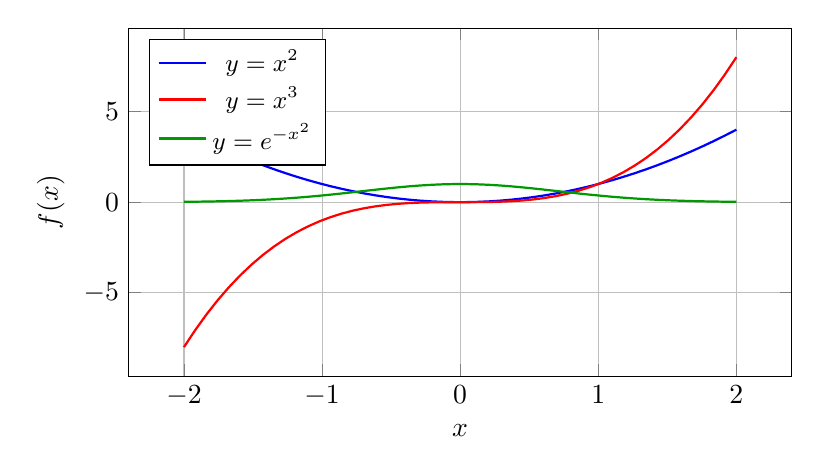
\begin{tikzpicture}
\begin{axis}[
  width=10cm, height=6cm,
  xlabel={$x$}, ylabel={$f(x)$},
  grid=major,
  legend pos=north west,
  legend style={font=\small}
]
\addplot[blue, thick, domain=-2:2, samples=50] {x^2};
\addlegendentry{$y = x^2$}
\addplot[red, thick, domain=-2:2, samples=50] {x^3};
\addlegendentry{$y = x^3$}
\addplot[green!60!black, thick, domain=-2:2, samples=50] {exp(-x^2)};
\addlegendentry{$y = e^{-x^2}$}
\end{axis}
\end{tikzpicture}
\end{center}
\end{example}

%% =============================================================================
%% Font Awesome 图标
%% =============================================================================
\clearpage
\section{Font Awesome 图标}

Font Awesome 5 提供了上千个矢量图标,可以让你的文档更加生动专业。

\subsection{常用图标速查}

\begin{table}[htbp]
\centering
\caption{常用图标}
\begin{tabular}{llllllll}
\toprule
图标 & 代码 & 图标 & 代码 & 图标 & 代码 & 图标 & 代码 \\
\midrule
\faHome & \verb|\faHome| & \faUser & \verb|\faUser| & \faEnvelope & \verb|\faEnvelope| & \faPhone & \verb|\faPhone| \\
\faSearch & \verb|\faSearch| & \faCog & \verb|\faCog| & \faCheck & \verb|\faCheck| & \faTimes & \verb|\faTimes| \\
\faGithub & \verb|\faGithub| & \faPython & \verb|\faPython| & \faRust & \verb|\faRust| & \faDocker & \verb|\faDocker| \\
\bottomrule
\end{tabular}
\end{table}

\subsection{信息提示框}

利用图标可以创建信息提示效果:

\begin{example}[图标与文字组合]
\begin{center}
\begin{tabular}{ll}
\textcolor{blue}{\faInfoCircle}\hspace{0.3em} 信息提示 & \verb|\faInfoCircle| \\
\textcolor{yellow!70!orange}{\faLightbulb}\hspace{0.3em} 小技巧 & \verb|\faLightbulb| \\
\textcolor{orange}{\faExclamationTriangle}\hspace{0.3em} 警告 & \verb|\faExclamationTriangle| \\
\textcolor{green!60!black}{\faCheckCircle}\hspace{0.3em} 成功 & \verb|\faCheckCircle| \\
\textcolor{red}{\faTimesCircle}\hspace{0.3em} 错误 & \verb|\faTimesCircle| \\
\end{tabular}
\end{center}
\end{example}

%% =============================================================================
%% LaTeX3 编程简介
%% =============================================================================
\clearpage
\section{LaTeX3 (expl3) 编程}

LaTeX3 是 \LaTeX{} 的现代化编程层,提供了一致的命名约定和强大的编程能力。

\subsection{命名约定}

expl3 使用 \verb|模块_函数:参数说明| 的命名格式:

\begin{table}[htbp]
\centering
\caption{expl3 模块简介}
\begin{tabular}{lll}
\toprule
模块 & 描述 & 示例 \\
\midrule
\verb|int| & 整数 & \verb|\int_step_inline:nn| \\
\verb|tl| & Token List & \verb|\tl_set:Nn| \\
\verb|str| & 字符串 & \verb|\str_if_eq:nnTF| \\
\verb|seq| & 序列 & \verb|\seq_push:Nn| \\
\verb|fp| & 浮点数 & \verb|\fp_eval:n| \\
\bottomrule
\end{tabular}
\end{table}

\subsection{xparse 文档命令}

\verb|xparse| 提供了灵活的命令定义方式:

\begin{table}[htbp]
\centering
\caption{xparse 参数类型}
\begin{tabular}{lll}
\toprule
类型 & 描述 & 示例用法 \\
\midrule
\verb|m| & 必选参数 & \verb|{内容}| \\
\verb|o| & 可选参数 & \verb|[选项]| \\
\verb|O{默认}| & 带默认值可选参数 & 省略时用默认值 \\
\verb|s| & 星号标记 & \verb|*| \\
\bottomrule
\end{tabular}
\end{table}

%% =============================================================================
%% 参考资源
%% =============================================================================
\clearpage
\section{参考资源}

\begin{itemize}
  \item[\faGlobe] \LaTeX{} 官方网站:\url{https://www.latex-project.org/}
  \item[\faBook] Overleaf 学习资源:\url{https://www.overleaf.com/learn}
  \item[\faCode] KaTeX 支持符号:\url{https://katex.org/docs/supported.html}
  \item[\faPalette] TikZ 示例库:\url{https://tikz.dev/}
  \item[\faIcons] Font Awesome 图标:\url{https://fontawesome.com/}
  \item[\faGithub] ElegantNote 模板:\url{https://github.com/ElegantLaTeX/ElegantNote}
\end{itemize}

\begin{center}
\begin{tikzpicture}
  \node[fill=ecolor!10, draw=ecolor, rounded corners=8pt, inner sep=12pt] {
    \faHeart\hspace{0.3em} \textbf{Happy \TeX{}ing!}
  };
\end{tikzpicture}
\end{center}

\end{document}
